% Template for PLoS
% Version 3.4 January 2017
\documentclass[10pt,letterpaper]{article}
\usepackage[top=0.85in,left=2.75in,footskip=0.75in]{geometry}

% amsmath and amssymb packages, useful for mathematical formulas and symbols
\usepackage{amsmath,amssymb}

% Use adjustwidth environment to exceed column width (see example table in text)
\usepackage{changepage}

% Use Unicode characters when possible
\usepackage[utf8x]{inputenc}

% textcomp package and marvosym package for additional characters
\usepackage{textcomp,marvosym}

% cite package, to clean up citations in the main text. Do not remove.
% \usepackage{cite}

% Use nameref to cite supporting information files (see Supporting Information section for more info)
\usepackage{nameref,hyperref}

% line numbers
\usepackage[right]{lineno}

% ligatures disabled
\usepackage{microtype}
\DisableLigatures[f]{encoding = *, family = * }

% color can be used to apply background shading to table cells only
\usepackage[table]{xcolor}

% array package and thick rules for tables
\usepackage{array}

% create "+" rule type for thick vertical lines
\newcolumntype{+}{!{\vrule width 2pt}}

% create \thickcline for thick horizontal lines of variable length
\newlength\savedwidth
\newcommand\thickcline[1]{%
  \noalign{\global\savedwidth\arrayrulewidth\global\arrayrulewidth 2pt}%
  \cline{#1}%
  \noalign{\vskip\arrayrulewidth}%
  \noalign{\global\arrayrulewidth\savedwidth}%
}

% \thickhline command for thick horizontal lines that span the table
\newcommand\thickhline{\noalign{\global\savedwidth\arrayrulewidth\global\arrayrulewidth 2pt}%
\hline
\noalign{\global\arrayrulewidth\savedwidth}}


% Remove comment for double spacing
%\usepackage{setspace} 
%\doublespacing

% Text layout
\raggedright
\setlength{\parindent}{0.5cm}
\textwidth 5.25in 
\textheight 8.75in

% Bold the 'Figure #' in the caption and separate it from the title/caption with a period
% Captions will be left justified
\usepackage[aboveskip=1pt,labelfont=bf,labelsep=period,justification=raggedright,singlelinecheck=off]{caption}
\renewcommand{\figurename}{Fig}

% Use the PLoS provided BiBTeX style
% \bibliographystyle{plos2015}

% Remove brackets from numbering in List of References
\makeatletter
\renewcommand{\@biblabel}[1]{\quad#1.}
\makeatother

% Leave date blank
\date{}

% Header and Footer with logo
\usepackage{lastpage,fancyhdr,graphicx}
\usepackage{epstopdf}
\pagestyle{myheadings}
\pagestyle{fancy}
\fancyhf{}
\setlength{\headheight}{27.023pt}
\lhead{
\includegraphics[width=2.0in]{PLOS-submission.eps}}
\rfoot{\thepage/\pageref{LastPage}}
\renewcommand{\footrule}{\hrule height 2pt \vspace{2mm}}
\fancyheadoffset[L]{2.25in}
\fancyfootoffset[L]{2.25in}
\lfoot{\sf PLOS}

%% Include all macros below
\newcommand{\lorem}{{\bf LOREM}}
\newcommand{\ipsum}{{\bf IPSUM}}





\usepackage{forarray}
\usepackage{xstring}
\newcommand{\getIndex}[2]{
  \ForEach{,}{\IfEq{#1}{\thislevelitem}{\number\thislevelcount\ExitForEach}{}}{#2}
}

\setcounter{secnumdepth}{0}

\newcommand{\getAff}[1]{
  \getIndex{#1}{Smith College}
}

\providecommand{\tightlist}{%
  \setlength{\itemsep}{0pt}\setlength{\parskip}{0pt}}

\begin{document}
\vspace*{0.2in}

% Title must be 250 characters or less.
\begin{flushleft}
{\Large
\textbf\newline{Classifying Socially Impactful Articles} % Please use "sentence case" for title and headings (capitalize only the first word in a title (or heading), the first word in a subtitle (or subheading), and any proper nouns).
}
\newline
\\
Julianna Alvord\textsuperscript{\getAff{Smith College}},
Minji Kang\textsuperscript{\getAff{Smith College}},
Zainab Rizvi\textsuperscript{\getAff{Smith College}},
Erina Fukuda\textsuperscript{\getAff{Smith College}}\\
\bigskip
\textbf{\getAff{Smith College}}Statistical \& Data Sciences, 1 Chapin Way Northampton, Massachusetts
01063\\
\bigskip
\end{flushleft}
% Please keep the abstract below 300 words
\section*{Abstract}
This project aims to find a way to classify socially impactful articles
based on social media and textual statustics. We trained three models
(tree, SVM and logistic regression) to have several approaches in
identifying socially impactful articles. Afterwards, we created a tool
through Shiny to create a friendly user-interface that displays the
results of these models plus an average of the three. By doing so, the
tool provides four scores. The scores serve as a simple guideline for
readers curious to know the probability of an article being socially
impactful simply by inputting a URL.

% Please keep the Author Summary between 150 and 200 words
% Use first person. PLOS ONE authors please skip this step. 
% Author Summary not valid for PLOS ONE submissions.   
\section*{Author summary}
We are students at Smith College enrolled in the SDS 410 Capstone course
in the Statistical \& Data Sciences Department.

\linenumbers

% Use "Eq" instead of "Equation" for equation citations.
\section{Introduction}\label{introduction}

Our team used articles from a major online news publication and tried to
create a tool that could automatically classify socially impactful
articles from those that are not based on several aspects of the
article. These aspects included the article's presence in social media
(e.g.~number of likes, shares, etc.), level of readability and the
sentiments associated with the words used.

We define socially impactful articles as those that change the readers'
way of thinking. It can also bring someone to take action or change the
way they act. Even if it does not make them change their views, if the
article leaves an impression or makes readers think it can also be a
socially impactful article as well. Therefore, some impacts that the
article can have on readers are changing the way they think, leaving an
impression, or reaffirming their ideas. It could also make readers
change their habits or actions based on what they have read. These
definitions were condensed into a flowchart that was used for future
classification (as seen below).

\begin{figure}
\centering
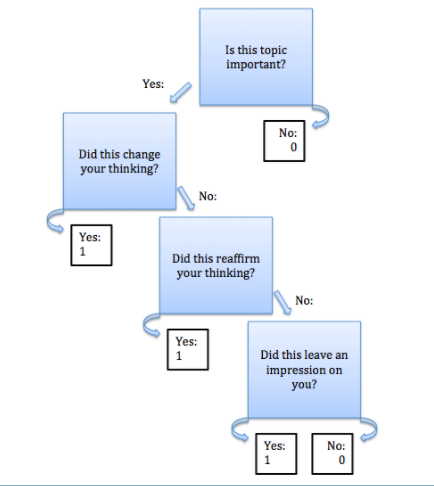
\includegraphics{tree.png}
\caption{}
\end{figure}

\section{Pre-existing Data}\label{pre-existing-data}

The data for this project were provided by the online news source which
contained information for their top 10000 most-viewed articles. This
news source collects and calculates data on many variables such as page
views, returning visitors, and social interactions for each of their
articles. The dataset given to us included 33 variables, the majority of
which were numeric. To understand these metrics, we referred to the
company's application programming interface (API) which contained a
description of 21 metrics. The API can be found at this address:
\url{https://www.parse.ly/help/api/available-metrics/}.

Other numeric metrics not included in this API were average views for
returning and new visitors, as well as direct, other, internal, and
search referrals. Direct referrals are a count of \ldots{}

The final six variables included the URL, title, publish date,
author(s), section, and tags. Example of tags are `ads\_scary' and
`health\_depression'. Some sections include `Crime', `Comedy',
`Entertainment', and `Politics'.

\subsection{Descriptive Statistics}\label{descriptive-statistics}

For this entire dataset of 10,000 observations, the average numbers of
page views was 105904.9. The average number of social interactions was
12957.97. An average of 77584.06 engaged minutes were spent on each
article. The top three sections were Politics (27.94\% of articles),
Entertainment (18.62 \%), and Comedy (4.86\%).

\subsection{Subsetting our Data}\label{subsetting-our-data}

While initially defining social impact, we discovered the difficulty of
comparing articles from different sections. For example, an article from
the entertainment section would never seem socially impactful when
compared to an article from a section like ``Black Voices.''

Existing literature also indicates that text mining models perform
better when they are domain-specific and that it is difficult to compare
results across different domains.

We decided that this project needed to start with only one section. The
section chosen was politics because it had the highest number of
articles which was 2,794.

\section{Collection of Additional
Data}\label{collection-of-additional-data}

\subsection{Text Mining}\label{text-mining}

We realized that all of our existing data tell us about the social media
reach of a given article. However, one of the problems specified by our
client was that social media reach is oftentimes not a good indicator of
whether the article is socially impactful or not. In order to add
another dimension to our data, we decided to retrieve the text of the
articles from the URLs that were provided to us in the dataset.

We wrote a Python script that takes in the URL as input and scrapes the
webpage to retrieve the text. We used the BeautifulSoup package in
Python for this purpose.

\section{Incorporating Natural Language Processing
Statistics}\label{incorporating-natural-language-processing-statistics}

We decided to supplement the social media statistics we got from our
client with some basic text mining statistics that give us some
information about the text. As discussed earlier, since the task at hand
is to judge the impact of the articles, we made the assumption that
there would be some relationship between the text itself and the impact
it creates.

We wrote a script in Python for this purpose using the textstat Python
package.The script takes as input the text of the articles (obtained
from the parser) and outputs the computed statistics. Specifically, we
calculate the following five statistics:

\begin{enumerate}
\def\labelenumi{\arabic{enumi}.}
\tightlist
\item
  word\_count: This calculates the number of words in the text.
\item
  sentence\_count: This calculates the number of sentences in the text.
\item
  readability\_score: This calculates the Flesch Reading Ease Score
  which is helpful to access the ease of readability in a document and
  ranges from 0 to 100 where 0 is difficult to read and 100 is easy to
  read.
\item
  grade\_level: This is calculated using the Automated Readability Index
  which outputs a number that approximates the grade level needed to
  comprehend the given text. This ranges from 1 to 12.
\item
  smog\_index: This calculates the a statistics called Simple Measure of
  Gobbledygook for the given text. In simple terms, smog index
  calculates the difficulty level of a sentences based on the number of
  words that are polysyllabic. It ranges from 5 to 22 which corresponds
  to the age of the reader who can understand the given text.
\end{enumerate}

\subsection{Article Classification}\label{article-classification}

In order to run supervised learning models, data collection was needed
to create the training set. Thus, we decided to unilize Amazon
Mechanical Turk (MTurk) for data collection to ensure the data was from
a random sample. MTurk is a crowdsourcing internet marketplace where
``Requesters'' create tasks that require human intelligence and
``Workers'' are paid upon successful completion of each task also known
as HITs (Human Intelligence Tasks).

As requesters, we launched tasks that provided a hyperlink to an article
and the flow chart that was previously created to help defined
classification of socially impactful articles. For each HIT the workers
were asked to click the hyperlink to be directed to the article, read
the article, and classify the articles after following the given flow
chart. We launched 2500 articles and requested 3 iterations of each
article. Thus, we had a total of 7500 HITs. Upon data collection,
analysis of the 7500 HITs was conducted. Pearson correlation of the
three iteration indicated that none of the interactions were even
slightly correlated to one another, implying that the results of the
classification of the articles were random. Another analysis was
conducted to test whether the correlation was statistically
significantly different from an actual random imputation of the
classification of the articles. The results indicated that the data
collected through MTurk was no different from random imputations.

Following the results of the first MTurk, we launched another set of
tasks that provided the parsed text of the article and same flow chart
from the pervious task. For each HIT the workers were asked to read the
parsed text, summarize the text in two to five sentences, and classify
the articles after following the given flow chart. This time, we
launched 500 articles with 3 iterations of each articles. Thus, we had a
total 1500 HITs. The results of the data collection had 97\% of the
articles rated as socially impactful. Thus, this data was discarded as
well.

Finally, the data collection was conducted by our group members going
through each articles and classifying the articles ourselves following
the flow chart we created. We classified a total of 900 articles and
used these 900 articles as the training set.

\section{Data Cleaning}\label{data-cleaning}

Once the NLP and sentiment analysis was completed, the original traffic
data of each articles and the new NLP and sentiment analysis as well as
the social impact classification outcome were complied together. In
order to build supervised learning models, only numerical vectors were
selected for data analysis. Thus variables such as \texttt{Tags},
\texttt{Published\_Date}, \texttt{Author} and the parsed \texttt{Text}
was removed. However we kept \texttt{URL} and \texttt{Title} variables,
but those were not included in the models. Additionally, six duplicated
rows were removed.

\subsection{Missing Data}\label{missing-data}

There were few missing entries in the traffic data given by our client.
Not all of the articles have been shared on every single media platform
which created missing entries within our data set. In order to account
for missing data of different social references and interaction with
social media of the articles, a dummy variable was created that
indicated whether the article has been shared in each of the different
social media platforms. On the other hand, all the articles have been
shared on Facebook and Twitter. Thus two new variables were created that
counted the interaction and references on other social media platform
than Facebook and Twitter. Lastly, 6 rows have been removed due to
missing NLP and sentiment analysis statistics as some articles did not
have any text and only included Twitter Threads or videos.

\subsection{Sentiment Analysis}\label{sentiment-analysis}

We used the \texttt{tidytext} package's \texttt{AFINN} lexicon for our
sentiment analysis. \texttt{AFINN} consists of around 2500 words and
phrases scored between -5 to +5. The number between 1 to 5 reflects the
severity of the word and the signs imply the positivity of the word.

We scraped the articles of its text, broke up the text into individual
words and omitted any commonly used words that should be ignored (e.g.
``the'', ``and'', ``is'') from the text. Then, the text was inspected
for words that fell into any of the 10 categories between -5 to +5 (0
was omitted). By using this method, we were able to add a column for -5
to -1 and +1 to +5 and label what percent of all words used in the
article (after taking out the stop words) fell into each category of
ratings. This was an effort to get an idea of what sentiments were
present in the article.

However, one limitation of this sentiment analysis is the fact that this
analysis was only done for one word each. Therefore, words that go
together may not be accounted for. In addition, the system is unable to
recognize the difference between word-usage depending on the context.
For example, if an article was referring to ``swift'' as a name, the
sentiment analysis will not be able to distinguish it from the adjective
``swift'' which is given a rating of +2. Therefore, the +2 word
percentage rate will increase due to the word usage in the text, even
though it is not part of the rating.

Overall, words rated higher on the scale of 1-5 (i.e. +5 and -5) were
not as prevalent in the articles, which makes sense given the
extremities of the words. The words were more common as the scales
became lower (i.e.~1-3).

-other data cleaning (MK?)

\subsection{MySQL database}\label{mysql-database}

Once we had the data cleaned, we uploaded it on the MySQL Server
database. Even though we are currently only working with 900 articles,
we wanted to make sure that our project is scalable. Putting the dataset
in a database also unified the schema for our different models.

\section{Models}\label{models}

\subsection{Decision Tree}\label{decision-tree}

Decision trees offer facilitated interpretation that is simple and easy
to understand. Decision trees provide comprehensive analysis of each
decision and partitions the data accordingly. We chose to use gradient
boosting as one of our model because it avoids over fitting. Boosting
reduces variance, unlike other decision tree models. Given a baseline
model, boosting fits a decision tree to the residuals from the baseline
model. Thus, Boosting grows trees sequentially allowing the next tree to
be fitted into a function to update their residuals. Since boosting
learns information from previous trees, the error rate is also usually
lower than other forest models.

Using the \texttt{caret} package in R, the gradient boosting model split
the data internally and ran its own training and testing models with
five cross validation folds. The model also tuned the parameter with
five cross validation folds. The optimal tuning parameters with the
highest Receiver Operating Characteristics (ROC = 0.807) was 650 trees
with shrinkage of 0.01, interaction depth of 3 and 9 minimum number of
observations in tree's terminal nodes. Thus, these parameters were used
for the final model. The gradient boosting model had an accuracy of
83.5\% and the 95\% confidence interval for accuracy was between 80.8\%
and 85.8\%. In addition the model also showed high sensitivity value of
0.918, but a lower specificity value of 0.692. Thus the model was
positively classifying impactful articles better than negatively
classifying impactful articles. The top 25 most important variables of
the boosting model results are shown in Figure X.

\subsection{Support Vector Machines}\label{support-vector-machines}

An SVM is a vector space based machine learning method where the goal is
to find a decision boundary between two classes that is maximally far
from any point in the training data (possibly discounting some points as
outliers or noise).

Our main motivation for using Support Vector Machines to classify the
articles was that SVMs are known to perform well in text classification
tasks, especially with small training sets. We use the e1071 package in
R and trained the SVM on 70\% training data from our classified
articles. When we predicted on the remaining 30\% of the data, we found
that the testing RMSE was 64\%.

After cross-validation and tuning, we found that a radial kernel
performs best on our data with a low cost and high gamma value.

A kernel is a compact representation of the similarity in the dataset.
Since we are working with multidimensional data, we tried linear,
polynomial, sigmoid and radial kernels to see which one gave the lowest
training RMSE.

We also iterated through different cost functions and realized that the
SVM performs the best with a low cost which means that there is a high
error on the training set compared to the testing set. We also had high
gamma parameter which indicates that there is high standard deviation
between the points.

We found that the ten most significant predictors for the SVM, in order
of significance, are:

\begin{enumerate}
\def\labelenumi{\arabic{enumi}.}
\tightlist
\item
  Total words
\item
  Visitors
\item
  Positivity score
\item
  Mobile views
\item
  Smog index
\item
  Grade level
\item
  Readability score
\item
  Returning visitors
\item
  Average minutes per new visitor
\item
  Negativity score
\end{enumerate}

\subsection{Logistic Regression. (to be changed due to changes in data +
variables/model)}\label{logistic-regression.-to-be-changed-due-to-changes-in-data-variablesmodel}

We fit a stepwise logistic regression as another measure to determine if
an article was socially impactful or not. The model included the
sentiment variables of -1 to -3 and +1 to +2, presence in social media
(i.e.~social interactions), smog index and length of the article
(i.e.~total number of words). All were significant (p-value \textless{}
0.05) and the model had a McFadden's R-squared of 0.143. In addition,
the logistic regression had an area under the curve of 0.820.

This model was cross-validated, and we noticed that the model had a
sensitivity of 0.47 but a specificity of 0.91. Therefore, it does a very
good job of classifying non-socially impactful articles but does not
perform well in classifying socially impactful articles. We are
currently working on first classifying non-socially impactful articles
using this logistic regression, then taking the articles classified as
``socially impactful'' and re-fitting another model for it for better
accuracy. We will need to be careful of overfitting, however, and we
should proceed with caution.

\subsection{Clustering}\label{clustering}

Since all the models we have used are supervised learning models that
train on numerical predictors, we also attempted unsupervised k-means
clustering to see if we could derive any insight from only using text as
a predictor. Our textual mining statistics convey important information
about the text of the articles but we were curious to see if there are
semantic differences that were not captured by numerical predictors.

We used k-means clustering using the nltk package in Python. K-means is
a clustering algorithm that classifies a given dataset around a
predefined k number of clusters.

Unfortunately, we found that the optimum number of clusters was 1 which
indicates that there were not meaningful distinctions between the group
of articles that we rated as socially impactful and the group of
articles we rates as not being socially impactful as they were all put
in the same cluster. The next optimum number of clusters was 8 but on
further investigation, we could not find a significant relationship
among the contents of each cluster and the assignment of socially
impactful articles to clusters was random. Therefore, we have decided
not to include clustering in our final ensemble model.

\subsection{Shiny App}\label{shiny-app}

\emph{Creation of Shiny App.} In order to display the results of our
models, a web application was created using the Shiny package in R. The
basic mechanism of the app starts with a user input of an article's URL.
In order for the app to correctly run, the URL must be one of the 891
found in our SQL table. From there, multiple models predict the
article's probability of social impact. Those probabilities are
averaged. The probabilities reactively change for each article.

\emph{Method.} Three of our models are displayed on the app: the
optimized boosting model, support vector machine model, and the multiple
logistic model. Each model was saved as R data (.rda) files. These files
were loaded into an r script at the top of the app file.

An important aspect of the app's server is the SQL query. First, the app
connects to the database. Within a reactive function from the Shiny
package, the politics table is exported, while filtering by the user
input URL. In order to query the title, the title column is selected
from table created in the initial reactive function, and transformed to
a dataframe. From there, this object is transformed into a vector to be
displayed on the app by the renderText function from the Shiny package.

\emph{Predicting in Shiny.} Within a renderText function, the title and
URL columns from the table created in the reactive function are removed.
This new table is used within the predict function to predict the
probability of social impact from each model. These numbers are then
added to vertical lines on the distributions.

\emph{Interface.} The app contains four rows. The top row contains the
title of the app, ``Is this Article Socially Impactful?'' The row below
contains a text input box that prompts the user to enter a URL as well
as a location for the title of the corresponds to appear. Below this, a
visualization using ggplot2 displays the distributions of probabilities
for each of the models. Once an article is entered, vertical lines
appear at the probabilities which are predicted by each model. The
fourth row displays the probabilities from the three models as well as
the average. The probabilities are each a different color that
coordinate with the distributions and vertical lines of the
visualization. A screenshot of the app is included below in figure 2.

\begin{figure}
\centering
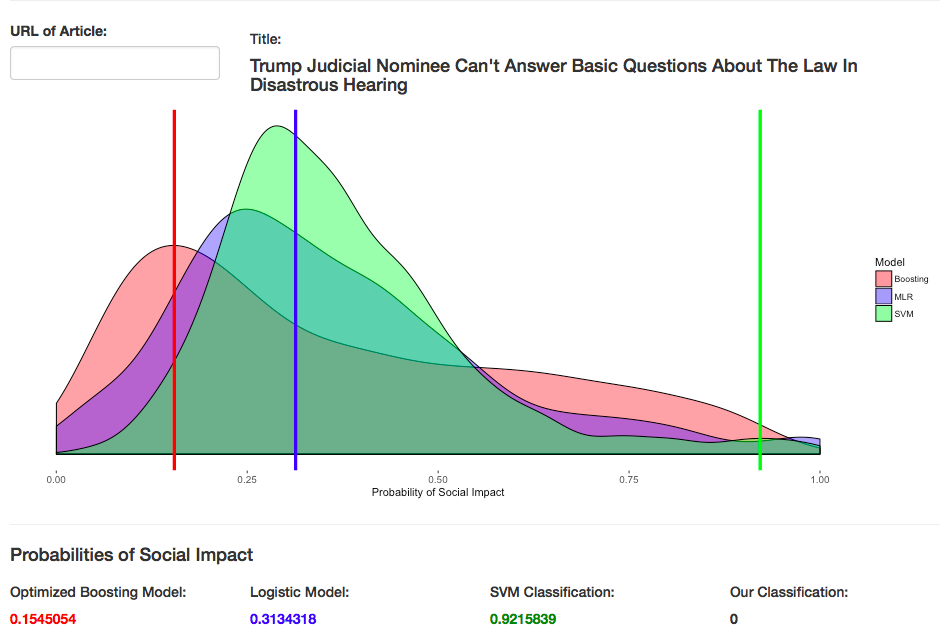
\includegraphics{Screen Shot 2018-04-19 at 9.47.35 AM.png}
\caption{}
\end{figure}

\section{Limitations \& Further
Discussion}\label{limitations-further-discussion}

There were various limitations to this study. Many of these limitations
are connected to our method of data collection. Because we rated the 900
articles ourselves, our data are not independent. Additionally, there is
a problem with bias in our data. Only four people were classifying, each
with similar educational backgrounds and . This group is not
representative of the entire population. For these reasons, the results
of this project are not generalizable.

Many of the variables in our model are connected and have high
correlations. For instance, the \texttt{social\ interactions} variable
is simply a summation of the facebook, twitter, pinterest, and linkedin
interactions. The models may be using variables like these that are
connected and causing inefficiencies.

Our choice to subset our data to only politics articles may also be
considered a limitation. Instead of being able to classify any article
from our news source, it is only appropriate to use our models to
classify Politics articles. Other sections may require different
variables to classify articles and our models cannot be generalized to
them.

Despite this limitation, our group made the decision that models which
classified an article from any section would not be productive. In this
case, there would likely be a high number of both type I and II errors.
Some, like politics articles for example, may be over-classified as
socially impactful whereas others, like comedy articles, may be
under-classified.

\section{Future Work}\label{future-work}

In the future, we hope to use other data collection methods to create a
training set for our models. Possibly, adjusting our flowchart then
utilizing AMT again may be one solution. We could also attempt to find
other individuals to classify a number of articles. To solve the issues
mentioned in the limitations section, this group would need to be larger
and hopefully more representative of the entire population of those who
read these articles.

We also plan on investigating the variables in our model and make
determinations of whether they are necessary and if there are any we
could exclude to simplify our models.

We also hope to expand our interface to other sections outside of
Politics too.

\section*{References}\label{references}
\addcontentsline{toc}{section}{References}

http://www2.imm.dtu.dk/pubdb/views/publication\_details.php?id=6010

\nolinenumbers


\end{document}

